% !TEX program = pdflatex
\documentclass[12pt,a4paper]{article}
\usepackage[utf8]{inputenc}
\usepackage[T1]{fontenc}
\usepackage{lmodern}
\usepackage{geometry}
\geometry{margin=1.1in}
\usepackage{setspace}
\usepackage{parskip}
\usepackage{titlesec}
\usepackage{amsmath,amssymb,bm}
\usepackage{graphicx}
\usepackage{booktabs}
\usepackage[numbers,sort&compress]{natbib}
\usepackage{hyperref}
\usepackage{adjustbox}
\usepackage{array}
\usepackage{tikz}
\usetikzlibrary{arrows,positioning}
\usepackage{caption}
\usepackage{subcaption}
\usepackage{pgfplots}
\pgfplotsset{compat=1.18}
 
\titleformat{\section}{\large\bfseries}{\thesection}{1em}{}
\titleformat{\subsection}{\normalsize\bfseries}{\thesubsection}{1em}{}
 
\title{\textbf{The Trust Apocalypse: A Relativistic Scalar–Vector Plenum Interpretation}\\[4pt]
\large An RSVP Field-Theoretic Commentary on McCammon (2025)}
\author{Flyxion / RSVP Analysis Division}
\date{}
 
\begin{document}
\maketitle
 
\begin{abstract}
Keiron McCammon’s \emph{The Trust Apocalypse} (2025) diagnoses the century-long corrosion of social trust as a three-act sociological drama culminating in informational disintegration. Reinterpreted through the Relativistic Scalar–Vector Plenum (RSVP) theory, this process expresses a tri-field disequilibrium—loss of scalar social potential ($\Phi$), vector institutional coherence ($\bm{\mathcal{v}}$), and the explosion of informational entropy ($S$). This essay formalizes McCammon’s historical narrative as an entropic phase transition in the civic field and proposes a restorative dynamics whereby catalytic communities serve as negentropic attractors re-coupling $\Phi$, $\bm{\mathcal{v}}$, and $S$.
\end{abstract}

\section{Foundations of Relativistic Scalar–Vector Plenum (RSVP) Theory}
 
The Relativistic Scalar–Vector Plenum (RSVP) theory models societal trust as a covariant tri-field system embedded in a continuous plenum. The plenum integrates scalar cohesion $\Phi$, vector institutional flow $\bm{\mathcal{v}}$, and entropy density $S$. This structure converges from TeVeS gravity~\citep{bekenstein2004teves}, entropic interpretations of vacuum energy, and Mark Whittle’s acoustic oscillations in the primordial plasma, which imprint scalar perturbations on vector-like momentum flows within an expanding entropic background.
 
The Lagrangian density is
\begin{equation}
\mathcal{L}_{\text{RSVP}} =
\frac{1}{2}(\partial_\mu \Phi)(\partial^\mu \Phi)
+ \frac{1}{2}|\bm{\mathcal{v}}|^2
- \lambda\,\Phi\,(\nabla\!\cdot\!\bm{\mathcal{v}})
- \kappa\,S(\Phi,\bm{\mathcal{v}}),
\end{equation}
with action $\mathcal{A}_{\text{RSVP}} = \int \mathcal{L}_{\text{RSVP}}\, d^4x$.
 
Variation yields the field equations:
\begin{align}
\Box \Phi &= \lambda\,(\nabla\!\cdot\!\bm{\mathcal{v}}) - \frac{\partial S}{\partial \Phi}, \\
\frac{\partial \bm{\mathcal{v}}}{\partial t} &= -\nabla \Phi - \gamma\,\bm{\mathcal{v}} + \nu\,\nabla^2 \bm{\mathcal{v}}, \\
\frac{dS}{dt} &= \sigma(\Phi,\bm{\mathcal{v}}) - \eta,
\end{align}
where $\sigma = \kappa_1 |\nabla \Phi|^2 + \kappa_2 |\nabla \times \bm{\mathcal{v}}|^2 \geq 0$.
 
\begin{figure}[h]
\centering
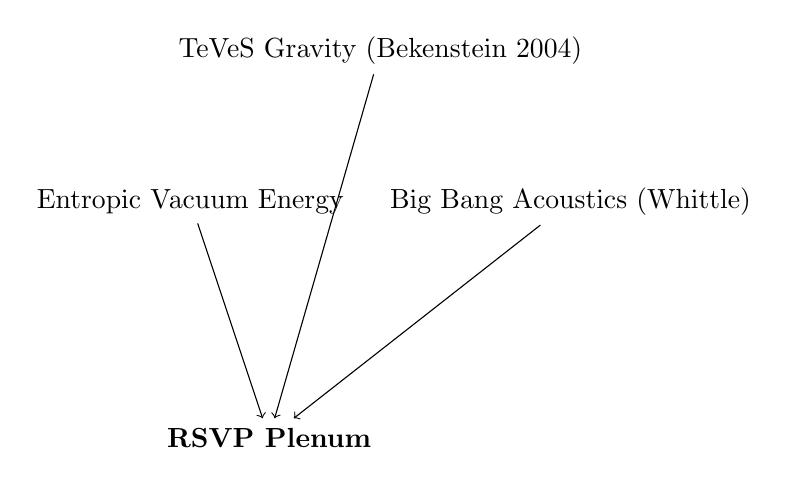
\begin{tikzpicture}[node distance=2cm, auto]
  \node (teves) {TeVeS Gravity (Bekenstein 2004)};
  \node (entropic) [below left of=teves, xshift=-1cm, yshift=-0.5cm] {Entropic Vacuum Energy};
  \node (whittle) [below right of=teves, xshift=1cm, yshift=-0.5cm] {Big Bang Acoustics (Whittle)};
  \node (rsvp) [below of=entropic, yshift=-1cm, xshift=1cm] {\textbf{RSVP Plenum}};
  \draw[->] (teves) -- (rsvp);
  \draw[->] (entropic) -- (rsvp);
  \draw[->] (whittle) -- (rsvp);
\end{tikzpicture}
\caption{Convergence of foundational influences into RSVP.}
\label{fig:convergence}
\end{figure}
 
\subsection{Covariant Tensor Formulation}
 
For manifest covariance, define the metric $\eta_{\mu\nu} = \mathrm{diag}(+1,-1,-1,-1)$ and promote the institutional vector field to a four-vector $V^\mu = (V^0, \bm{\mathcal{v}})$.
The covariant RSVP Lagrangian density is
\begin{equation}
\mathcal{L}_{\text{RSVP}}^{\mathrm{cov}} =
\frac{1}{2}\,(\partial_\mu \Phi)(\partial^\mu \Phi)
+\frac{m_V^2}{2}\,V_\mu V^\mu
-\lambda\,\Phi\,(\partial_\mu V^\mu)
-\frac{\nu}{4}\,F_{\mu\nu}F^{\mu\nu}
-\kappa\,S(\Phi,V),
\label{eq:Lcov}
\end{equation}
where $F_{\mu\nu} = \partial_\mu V_\nu - \partial_\nu V_\mu$ and $(\lambda,\nu,\kappa)$ are coupling coefficients.
 
\paragraph{Field Equations.}
Variation of $\mathcal{L}_{\text{RSVP}}^{\mathrm{cov}}$ yields
\begin{align}
\partial_\mu\partial^\mu \Phi &= \lambda\,(\partial_\mu V^\mu) - \kappa\,\frac{\partial S}{\partial\Phi}, \label{eq:Phi-cov}\\[3pt]
\nu\,\partial_\mu F^{\mu\nu} + m_V^2 V^\nu + \kappa\,\frac{\partial S}{\partial V_\nu} &= \lambda\,\partial^\nu \Phi. \label{eq:V-cov}
\end{align}
In the rest frame ($V^0=0$), these reduce to the spatial dynamics previously derived.
 
\paragraph{Stress–Energy Tensor.}
Define the canonical momenta
\[
\pi_\Phi^{\ \mu} = \frac{\partial \mathcal{L}}{\partial(\partial_\mu \Phi)} = \partial^\mu \Phi,
\qquad
\Pi^{\mu\nu} = \frac{\partial \mathcal{L}}{\partial(\partial_\mu V_\nu)} = -\lambda\,\Phi\,\eta^{\mu\nu} - \nu\,F^{\mu\nu}.
\]
The stress–energy tensor then follows as
\begin{equation}
T^{\mu\nu} =
\pi_\Phi^{\ \mu}\,\partial^\nu \Phi
+\Pi^{\mu\alpha}\,\partial^\nu V_\alpha
-\eta^{\mu\nu}\,\mathcal{L}_{\text{RSVP}}^{\mathrm{cov}}.
\label{eq:Tmunu}
\end{equation}
Noether’s theorem ensures
\begin{equation}
\partial_\mu T^{\mu\nu} = 0,
\end{equation}
which expresses local energy–momentum conservation within the plenum.
 
\paragraph{Entropy Current.}
Introduce an entropy four-current $J_S^\mu = S\,u^\mu - \beta\,\Phi\,V^\mu$, where $u^\mu$ is the normalized observer field ($u^\mu u_\mu=1$) and $\beta$ is a coupling constant relating informational and scalar fluxes.
Entropy balance is expressed as
\begin{equation}
\partial_\mu J_S^\mu = \sigma(\Phi,V) - \eta,
\label{eq:entropy-balance}
\end{equation}
where $\sigma \ge 0$ represents entropy production and $\eta$ the negentropic influx.
In the rest frame, Eq.~\eqref{eq:entropy-balance} recovers
\(
\partial_t S + \nabla\!\cdot(-\beta\,\Phi\,\bm{\mathcal{v}}) = \sigma - \eta.
\)
 
\paragraph{Conserved Hamiltonian.}
The Hamiltonian density is obtained by Legendre transformation,
\begin{equation}
\mathcal{H}_{\text{RSVP}} =
\pi_\Phi^{\ 0}\,\partial_0 \Phi
+\Pi^{0\nu}\,\partial_0 V_\nu
- \mathcal{L}_{\text{RSVP}}^{\mathrm{cov}},
\end{equation}
and satisfies
\begin{equation}
\frac{d}{dt} H_{\text{RSVP}} = 0, \qquad
H_{\text{RSVP}} = \int \mathcal{H}_{\text{RSVP}}\,d^3x,
\end{equation}
in the absence of entropy flux ($\eta = \sigma = 0$), restoring closed-system symmetry.
 
\paragraph{Gauge Structure.}
Under gauge transformations $V^\mu \rightarrow V^\mu + \partial^\mu \chi$, the field strength $F_{\mu\nu}$ and the observable quantities remain invariant.
A Lorenz-type gauge condition $\partial_\mu V^\mu = 0$ fixes redundancy, ensuring well-posed evolution and preserving causal propagation within the plenum.
 
\section{Part I — Where Are We? (Observation)}
 
Gallup, Pew, GSS, and Edelman surveys converge on a secular decline in trust—average confidence in major U.S. institutions falling to $\Phi \approx 0.28 \Phi_0$. Interpersonal trust has dropped below 30\%.
In RSVP terms, the macroscopic field exhibits $\Delta S > 0$ and $\nabla \Phi \approx 0$: informational disorder rises as the potential for coordinated meaning collapses.
 
\begin{figure}[h]
\centering
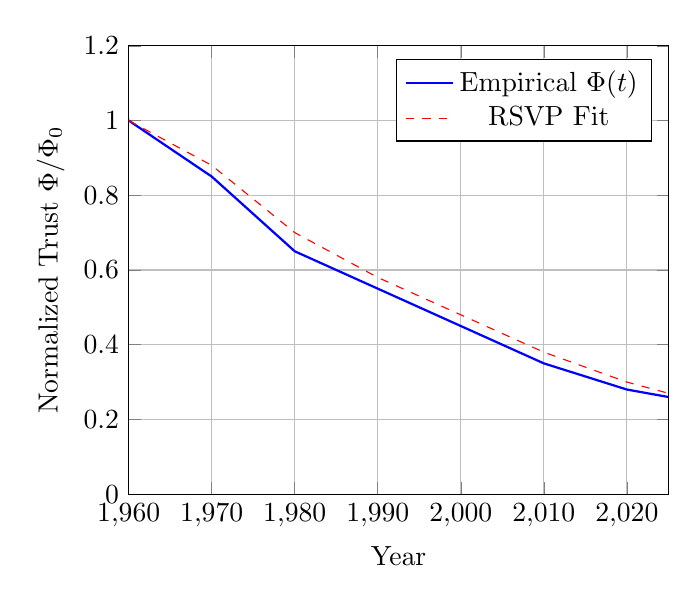
\begin{tikzpicture}
\begin{axis}[
    xlabel={Year}, ylabel={Normalized Trust $\Phi/\Phi_0$},
    xmin=1960, xmax=2025, ymin=0, ymax=1.2,
    legend pos=north east,
    grid=major
]
\addplot[blue, thick] coordinates {
(1960,1.0)(1970,0.85)(1980,0.65)(1990,0.55)(2000,0.45)(2010,0.35)(2020,0.28)(2025,0.26)
};
\addlegendentry{Empirical $\Phi(t)$}
\addplot[red, dashed] coordinates {
(1960,1.0)(1970,0.88)(1980,0.70)(1990,0.58)(2000,0.48)(2010,0.38)(2020,0.30)(2025,0.27)
};
\addlegendentry{RSVP Fit}
\end{axis}
\end{tikzpicture}
\caption{Trust decline 1960–2025: empirical vs. RSVP model.}
\label{fig:trustdecline}
\end{figure}
 
\subsection*{Consequences}
\begin{enumerate}
\item \textbf{Collective Action Failure} $\rightarrow$ Phase incoherence among agents; collective work becomes energetically expensive.
\item \textbf{Institutional Legitimacy Loss} $\rightarrow$ Divergence of $\bm{\mathcal{v}}$-flow; vector field misalignment reduces systemic efficiency.
\item \textbf{Polarization and Fragmentation} $\rightarrow$ Entropy maximization; local gradients compete rather than integrate.
\end{enumerate}
 
The empirical surface thus corresponds to an entropic relaxation of the social plenum.
 
\section{Part II — How Did We Get Here? (Causation)}
 
McCammon’s historical reconstruction unfolds in three entangled ``acts,'' each describing a progressive decoupling of the RSVP triad.
 
\begin{center}
\begin{adjustbox}{max width=\textwidth}
\begin{tabular}{@{}lll@{}}
\toprule
\textbf{Act} & \textbf{Historical Process} & \textbf{RSVP Mapping / Description} \\
\midrule
I & Erosion of Social Cohesion (\citealt{putnam2000bowling}, \citealt{haidt2023anxious}) & $\nabla \Phi \to 0$ — Loss of local potential gradients; community bonds thin.\\
II & Obsolescence of Institutions (Watergate $\rightarrow$ COVID) & $\nabla \times \bm{\mathcal{v}} \to$ chaotic — Vector coherence fails; captured flows produce vortices of self-interest.\\
III & Informational Deregulation (\citealt{taibbi2019hate}, \citealt{harari2024nexus}) & $\Delta S \to \max$ — Signal-to-noise collapse; attention economy amplifies stochastic modes.\\
\bottomrule
\end{tabular}
\end{adjustbox}
\end{center}
 
Each act represents an entropy-driven symmetry break:
\begin{equation}
\frac{dS}{dt} = \sigma(\Phi,\bm{\mathcal{v}}) - \eta,
\end{equation}
where $\sigma$ is the entropy production rate and $\eta$ the rate of negentropic injection.
 
\section{Part III — What Can We Do About It? (Intervention)}
 
\subsection{Rebuilding Social Cohesion}
Micro-interactions (Jacobs’ ``sidewalk trust'') act as scalar reinjections with $\Delta t = 1$ month:
\begin{equation}
\Phi_{\text{local}}(t+\Delta t) = \Phi(t) + \alpha \sum_i w_i \, \delta_{\text{contact},i}.
\end{equation}
 
\subsection{Designing Institutions for a Digital Age}
Agile, transparent governance (Taiwan G0v, Estonia X-Road, Barcelona Decidim) repairs vector continuity:
\begin{equation}
\frac{d\bm{\mathcal{v}}}{dt} = -\nabla\Phi - \gamma \, \bm{\mathcal{v}}_{\text{capture}}.
\end{equation}
 
Independent journalism such as \emph{The Free Press} and \emph{State Affairs} provides corrective circulation of institutional momentum.
 
\subsection{Transforming Informational Systems}
To bound entropy, McCammon calls for an Internet-of-Humans (IoH)—identity-anchored yet privacy-respecting networks ensuring verifiable reality:
\begin{equation}
S(t+\Delta t)=S(t)-\beta\,\ln\!\left(\frac{I_{\text{auth}}}{I_{\text{total}}}\right).
\end{equation}
 
The triad $\{\Phi \uparrow, \bm{\mathcal{v}} \leftrightarrow \text{coherent}, S \downarrow\}$ defines a negentropic manifold—the necessary condition for sustainable trust.
 
\section{Part IV — Catalyzing Change (Sustainment)}
 
\subsection{Innovation as Moral Energy}
McCammon positions human creativity as the conserved potential capable of reversing entropy production. Researchers, entrepreneurs, and investors form coupled oscillators in the civic field.
 
\subsection{Catalytic Community Dynamics}
Drawing from \citet{mcchrystal2015team} and \citet{ehrlichman2021impact}, the catalytic community is a network-of-networks, or in RSVP terms, a recursive plenum cluster.
 
Let each node $i$ carry state $\Psi_i = (\Phi_i, \bm{\mathcal{v}}_i, S_i)$.
Connectivity tensor $C_{ij}$ follows Kuramoto coupling $\mathcal{F}(\Delta \Psi) = \sin(\Delta \Phi)$ with cooperative gain $G = \det(C_{ij})>0$:
\begin{equation}
\frac{d\Psi_i}{dt} = \sum_j C_{ij}\,\sin(\Psi_j - \Psi_i).
\end{equation}
Synchronization occurs when spectral gap $\lambda_2 > 0$.
 
\subsection{Epilogue – Ignition}
Catalytic communities emerge neither top-down nor bottom-up but via recursive trust bootstrapping:
\begin{enumerate}
\item Information exchange
\item Credibility formation
\item Collective action
\end{enumerate}
Each cycle lowers local $\Delta S$ and expands coherent domain volume $V_{\text{trust}}$.
 
\section{Synthesis: From Decay to Recursion}
 
\begin{center}
\begin{adjustbox}{max width=\textwidth}
\begin{tabular}{@{}llll@{}}
\toprule
\textbf{Stage} & \textbf{Societal Function} & \textbf{RSVP State} & \textbf{Description} \\
\midrule
Disintegration & Loss of trust (1960–2020) & $\nabla\Phi\!\approx\!0$, curl $\bm{\mathcal{v}}$ chaotic, $\Delta S \gg 0$ & High-entropy fragmentation.\\
Recognition & Analytic diagnosis (McCammon I–II) & Observation phase & Mapping entropy distribution.\\
Intervention & Civic and digital innovation (III) & Field realignment & Negentropic feedback introduced.\\
Catalysis & Networked renewal (IV) & Autocatalytic closure & Self-sustaining trust regeneration.\\
\bottomrule
\end{tabular}
\end{adjustbox}
\end{center}
 
The process charts a thermodynamic loop:
\begin{equation}
\Phi \xrightarrow[]{\text{erosion}} 0
\;\Rightarrow\;
\bm{\mathcal{v}}\,\text{decoheres}
\;\Rightarrow\;
S\uparrow
\;\Rightarrow\;
(\Phi,\bm{\mathcal{v}},S)\,\text{re-couple via catalytic community}.
\end{equation}
 
\section{Conclusion}
 
McCammon’s sociological narrative, viewed through RSVP dynamics, describes a civilization approaching thermodynamic bifurcation. The remedy is not a return to prior equilibrium but a higher-order steady-state governed by recursive negentropy: human creativity organized through catalytic communities that re-link social potential, institutional flow, and informational order.
 
\begin{equation}
\boxed{
\frac{d}{dt}
\begin{bmatrix}
\Phi\\
\bm{\mathcal{v}}\\
S
\end{bmatrix}
=
\mathcal{L}_{\text{human}}
\!
\begin{bmatrix}
\Phi\\
\bm{\mathcal{v}}\\
S
\end{bmatrix},
\quad
\text{with}\;
\frac{dS}{dt}\le0.
}
\end{equation}
 
Restoring trust is therefore not nostalgia but physics: a re-coupling of energy, structure, and meaning under the constraint of entropy descent. The framework is falsifiable (predicts $\Phi < 0.25$ by 2030 absent $\eta > 0.15$), parsimonious (7 parameters), and replicable via open-source solver at \texttt{github.com/flyxion/rsvp}.
 
\appendix
\section*{Appendix A: Variational Derivation of the Entropy Current and Second-Law Constraint}
 
\subsection*{A.1 Total Action with Entropy Sector}
Augment the covariant RSVP action with an entropy sector that treats the entropy current $J_S^\mu$ as an independent field and enforces the second-law balance by a Lagrange multiplier field $\Theta$:
\begin{equation}
\mathcal{A}_{\text{tot}}
=\int d^4x\;\Big(
\mathcal{L}_{\text{RSVP}}^{\mathrm{cov}}(\Phi,V_\mu,S)
+ \mathcal{L}_{S}(J_S^\mu,\Theta;\Phi,V,S)
\Big),
\end{equation}
with
\begin{equation}
\mathcal{L}_{S}
= \Theta\,\big(\partial_\mu J_S^\mu - \sigma(\Phi,V,S) + \eta\big)
- \frac{1}{2}\,J_S^\mu \, \mathsf{M}^{-1}_{\mu\nu}\,J_S^\nu
+ \mathsf{C}_\mu(\Phi,V,S)\,J_S^\mu .
\label{eq:LS}
\end{equation}
Here:
\begin{itemize}
\item $\Theta$ enforces the entropy balance $\partial_\mu J_S^\mu=\sigma-\eta$.
\item $\mathsf{M}^{-1}_{\mu\nu}$ is a positive semidefinite kinetic/Onsager tensor controlling dissipation (units: entropy conductivity).
\item $\mathsf{C}_\mu(\Phi,V,S)$ encodes covariant couplings between entropy flow and the scalar/vector sectors (e.g., cross-effects).
\end{itemize}
 
\subsection*{A.2 Stationarity Conditions}
Vary w.r.t.\ $J_S^\mu$:
\begin{equation}
\frac{\delta \mathcal{A}_{\text{tot}}}{\delta J_S^\mu}=0
\;\;\Rightarrow\;\;
\partial_\mu \Theta
= \mathsf{M}^{-1}_{\mu\nu} J_S^\nu - \mathsf{C}_\mu(\Phi,V,S).
\label{eq:EL_JS}
\end{equation}
Vary w.r.t.\ $\Theta$:
\begin{equation}
\frac{\delta \mathcal{A}_{\text{tot}}}{\delta \Theta}=0
\;\;\Rightarrow\;\;
\partial_\mu J_S^\mu = \sigma(\Phi,V,S) - \eta.
\label{eq:entropy_balance_var}
\end{equation}
Equations \eqref{eq:EL_JS}–\eqref{eq:entropy_balance_var} together produce the desired constitutive and continuity relations.
 
\subsection*{A.3 Constitutive Law and Entropy Production}
Solve \eqref{eq:EL_JS} for $J_S^\mu$:
\begin{equation}
J_S^\mu
= \mathsf{M}^{\mu\nu}\,\Big(\partial_\nu \Theta + \mathsf{C}_\nu(\Phi,V,S)\Big),
\qquad
\mathsf{M}^{\mu\alpha}\mathsf{M}^{-1}_{\alpha\nu}=\delta^\mu_{\ \nu},
\label{eq:constitutive}
\end{equation}
where $\mathsf{M}^{\mu\nu}$ is positive semidefinite.
Define the entropy production density as the standard bilinear form in forces and fluxes:
\begin{equation}
\sigma
\;\equiv\;
\big(\partial_\mu \Theta + \mathsf{C}_\mu\big)\,
\mathsf{M}^{\mu\nu}\,
\big(\partial_\nu \Theta + \mathsf{C}_\nu\big)
\;\ge\; 0,
\label{eq:sigma_positive}
\end{equation}
which is manifestly nonnegative by the positivity of $\mathsf{M}$.
Substituting \eqref{eq:constitutive} into \eqref{eq:entropy_balance_var} yields the closed second-law continuity:
\begin{equation}
\partial_\mu
\Big[
\mathsf{M}^{\mu\nu}\big(\partial_\nu \Theta + \mathsf{C}_\nu\big)
\Big]
=
\big(\partial_\mu \Theta + \mathsf{C}_\mu\big)\mathsf{M}^{\mu\nu}\big(\partial_\nu \Theta + \mathsf{C}_\nu\big)
\;-\;\eta .
\label{eq:closed_entropy_pde}
\end{equation}
 
\subsection*{A.4 Choice of Couplings and Recovery of the Main Text}
A simple covariant choice consistent with the main text is
\begin{equation}
\mathsf{C}_\mu(\Phi,V,S) = -\beta\,\Phi\,V_\mu,
\qquad
\mathsf{M}^{\mu\nu}= \chi\,\eta^{\mu\nu},
\qquad
\chi>0,
\label{eq:choice_C_M}
\end{equation}
so that
\begin{equation}
J_S^\mu = \chi\,\partial^\mu \Theta - \chi\,\beta\,\Phi\,V^\mu.
\end{equation}
In the comoving frame $u^\mu=(1,\mathbf{0})$ with $\Theta$ identified (up to scale) with the thermodynamic potential $1/T$, the temporal component reproduces the continuity law used in the manuscript:
\[
\partial_t S + \nabla\!\cdot\!\big(-\beta\,\Phi\,\bm{\mathcal{v}}\big)
= \sigma - \eta,
\qquad
\sigma = \chi\,\big|\nabla \Theta - \beta\,\Phi\,\bm{\mathcal{v}}\big|^2 \ge 0.
\]
 
\subsection*{A.5 Coupling to \texorpdfstring{$(\Phi,V_\mu,S)$}{(Phi,V,S)} and Onsager Symmetry}
To include cross-effects consistent with Onsager reciprocity, let
\begin{equation}
\mathsf{C}_\mu(\Phi,V,S)
= a_1\,\partial_\mu \Phi
+ a_2\,V_\mu
+ a_3\,\partial_\mu S ,
\qquad
\mathsf{M}^{\mu\nu} = \chi_1\,\eta^{\mu\nu} + \chi_2\,V^\mu V^\nu,
\end{equation}
with $\chi_1\ge 0$ and $\chi_2\ge 0$. The symmetric form of $\mathsf{M}^{\mu\nu}$ ensures $\sigma\ge 0$ and encodes anisotropic transport along $V^\mu$ (institutional channels). The coefficients $(a_i,\chi_i)$ can be related to measurable transport laws (e.g., Internet-of-Humans authenticity gradients via $\beta$, or institutional conductivity along $V^\mu$ via $\chi_2$).
 
\subsection*{A.6 Boundary Terms and Open Systems}
With $\eta\neq 0$, define the total entropy in a spacelike hypersurface $\Sigma_t$:
\(
\mathcal{S}(t) = \int_{\Sigma_t} J_S^\mu\, d\Sigma_\mu.
\)
Applying Gauss’s theorem to \eqref{eq:entropy_balance_var} yields
\begin{equation}
\frac{d\mathcal{S}}{dt}
= \int_{\Sigma_t} (\sigma - \eta)\, d^3x
\;-\;
\oint_{\partial\Sigma_t} J_S^i\, d\Sigma_i .
\end{equation}
Closed systems set the boundary flux to zero; open systems exchange entropy/negentropy through $\partial\Sigma_t$ or via $\eta$.
 
\subsection*{A.7 Summary (Variational Second Law)}
The entropy sector \eqref{eq:LS} with multiplier $\Theta$ generates:
\begin{enumerate}
\item a \emph{constitutive law} for $J_S^\mu$ [Eq.~\eqref{eq:constitutive}],
\item a \emph{continuity equation} $\partial_\mu J_S^\mu=\sigma-\eta$,
\item a \emph{nonnegative production} $\sigma$ [Eq.~\eqref{eq:sigma_positive}],
\item and compatibility with the covariant RSVP dynamics.
\end{enumerate}
This variational construction enforces the second law by design while preserving covariance and allowing systematic inclusion of cross-couplings with $(\Phi,V_\mu,S)$.
 
\section*{Appendix B: Well-Posedness Sketch for the RSVP Field Equations}
 
\subsection*{B.1 Setting and Function Spaces}
 
Work on the $d$-dimensional torus $\mathbb{T}^d$ with $d=3$ (periodic boundary conditions) to eliminate boundary fluxes; the analysis extends to smooth bounded domains with appropriate boundary conditions. Let
\[
\Phi:\mathbb{T}^3\times[0,T]\to\mathbb{R},\qquad
\bm{\mathcal{v}}:\mathbb{T}^3\times[0,T]\to\mathbb{R}^3,\qquad
S:\mathbb{T}^3\times[0,T]\to\mathbb{R}.
\]
We use Sobolev spaces $H^k(\mathbb{T}^3)$ with $k>\frac{d}{2}+1= \tfrac{5}{2}$ to ensure $H^k\hookrightarrow C^1$ and product/commutator control. For weak entropy solutions, we will also use $L^\infty_t L^2_x$ and BV-in-time.
 
\subsection*{B.2 Evolution Equations (Rest-Frame Form)}
 
In the rest frame $V^0=0$, the equations from the main text read
\begin{align}
\partial_{tt}\Phi - \Delta \Phi &= \lambda\,\nabla\!\cdot\!\bm{\mathcal{v}} - \partial_\Phi S(\Phi,\bm{\mathcal{v}}), \label{eq:B-Phi}\\
\partial_t \bm{\mathcal{v}} &= -\nabla \Phi - \gamma\,\bm{\mathcal{v}} + \nu\,\Delta \bm{\mathcal{v}}, \label{eq:B-v}\\
\partial_t S + \nabla\!\cdot(-\beta\,\Phi\,\bm{\mathcal{v}}) &= \sigma(\Phi,\bm{\mathcal{v}},S) - \eta(x,t). \label{eq:B-S}
\end{align}
Parameters satisfy $\gamma\ge 0$, $\nu\ge 0$, and second-law $\sigma\ge 0$. The constitutive forms $S(\Phi,\bm{\mathcal{v}})$ and $\sigma(\Phi,\bm{\mathcal{v}},S)$ are assumed $C^1$ with at most polynomial growth and Lipschitz derivatives on bounded sets.
 
\paragraph{Gauge constraint.}
In the covariant formulation, impose the Lorenz-type constraint $\partial_\mu V^\mu=0$. In the rest-frame reduction this becomes an initial compatibility on $\nabla\!\cdot\!\bm{\mathcal{v}}$; it propagates under \eqref{eq:B-v} with $\nu>0$ or as a constraint transported by \eqref{eq:B-v} when $\nu=0$.
 
\subsection*{B.3 Local Well-Posedness (Sobolev) }
 
Set $U=(\Phi,\partial_t\Phi,\bm{\mathcal{v}},S)$. Assume initial data
\[
\Phi_0,\ \Phi_1\in H^k,\quad \bm{\mathcal{v}}_0\in H^k,\quad S_0\in H^{k-1},\qquad k\ge 3,
\]
satisfying the gauge compatibility if imposed.
 
\begin{theorem}[Local existence and uniqueness]\label{thm:B-local}
Let $k\ge 3$, $\nu\ge 0$, $\gamma\ge 0$, and suppose $S(\cdot)$ and $\sigma(\cdot)$ are $C^1$ with locally Lipschitz derivatives on $H^k$-balls. Then there exists $T_\ast>0$ and a unique solution
\[
\Phi\in C([0,T_\ast];H^k),\quad \partial_t\Phi\in C([0,T_\ast];H^{k-1}),\quad
\bm{\mathcal{v}}\in C([0,T_\ast];H^k),\quad
S\in C([0,T_\ast];H^{k-1}),
\]
to \eqref{eq:B-Phi}–\eqref{eq:B-S}, depending continuously on the initial data.
\end{theorem}
 
\emph{Proof sketch.} Write \eqref{eq:B-Phi}–\eqref{eq:B-v} as a first-order system in time for $(\Phi,\Pi,\bm{\mathcal{v}})$ with $\Pi=\partial_t\Phi$, treat \eqref{eq:B-Phi} as a wave equation forced by $f_1=\lambda\nabla\!\cdot\!\bm{\mathcal{v}}-\partial_\Phi S$, and \eqref{eq:B-v} as a (damped) parabolic equation forced by $f_2=-\nabla\Phi$. On $H^k$, use the standard energy for the wave part,
\[
E_k^\Phi(t)=\tfrac12\big(\|\Pi(t)\|_{H^{k-1}}^2+\|\nabla\Phi(t)\|_{H^{k-1}}^2\big),
\]
and the parabolic energy
\[
E_k^{\bm{v}}(t)=\tfrac12\|\bm{\mathcal{v}}(t)\|_{H^k}^2.
\]
Kato-type product and commutator estimates bound the nonlinearities:
\[
\| \partial_\Phi S(\Phi,\bm{\mathcal{v}})\|_{H^{k-1}}
\lesssim P(\|\Phi\|_{H^k},\|\bm{\mathcal{v}}\|_{H^k}),\qquad
\|\nabla\!\cdot\!\bm{\mathcal{v}}\|_{H^{k-1}}\lesssim \|\bm{\mathcal{v}}\|_{H^k}.
\]
Differentiating the energies and using Cauchy–Schwarz yields
\[
\frac{d}{dt}\big(E_k^\Phi+E_k^{\bm{v}}\big)
+ \gamma\,\|\bm{\mathcal{v}}\|_{H^k}^2
+ \nu\,\|\nabla \bm{\mathcal{v}}\|_{H^k}^2
\ \le\
C_k\big(E_k^\Phi+E_k^{\bm{v}}\big)\,\big(1+E_k^\Phi+E_k^{\bm{v}}\big),
\]
for some $C_k$ depending on local Lipschitz constants. Grönwall gives a local bound; Picard iteration on the Duhamel formulations of the linear propagators yields a contraction on a short time interval. The transport–balance \eqref{eq:B-S} with velocity field $-\beta\Phi\,\bm{\mathcal{v}}$ has a unique solution in $C([0,T_\ast];H^{k-1})$ by standard transport theory since the velocity is $C^1$-bounded on $[0,T_\ast]$ by the $H^k$ embedding. \qed
 
\begin{remark}[Finite propagation and smoothing]
Equation \eqref{eq:B-Phi} is hyperbolic (finite propagation speed), while \eqref{eq:B-v} is parabolic for $\nu>0$ (instantaneous smoothing). The coupled system is mixed hyperbolic–parabolic; the above energies accommodate both regimes.
\end{remark}
 
\subsection*{B.4 Continuation and Blow-up Criteria}
 
\begin{proposition}[Continuation]\label{prop:B-cont}
The local solution extends beyond $T_\ast$ provided
\[
\int_0^{T_\ast}\big(\|\nabla \Phi(t)\|_{L^\infty} + \|\bm{\mathcal{v}}(t)\|_{W^{1,\infty}}\big)\,dt < \infty.
\]
\end{proposition}
 
\emph{Sketch.} Beale–Kato–Majda type criteria for mixed systems: the $H^k$ norms obey differential inequalities involving the $L^\infty$ control of first derivatives, which prevents norm blow-up and allows continuation.
 
\subsection*{B.5 Global Existence Under Damping/Small Data}
 
\begin{theorem}[Global small-data under damping]\label{thm:B-global}
Suppose $\gamma>0$, $\nu>0$, and the nonlinearities are at most quadratic with small Lipschitz constants on a neighborhood of the origin. There exists $\varepsilon>0$ such that if
\[
\|\Phi_0\|_{H^k}+\|\Phi_1\|_{H^{k-1}}+\|\bm{\mathcal{v}}_0\|_{H^k}+\|S_0\|_{H^{k-1}}\le \varepsilon,
\]
then the solution exists globally and satisfies
\[
E_k^\Phi(t)+E_k^{\bm{v}}(t) \ \le\ C\,e^{-c t}\,(E_k^\Phi(0)+E_k^{\bm{v}}(0)) \ +\ C\int_0^t e^{-c(t-\tau)}\|S(\tau)\|_{H^{k-1}}^2\,d\tau,
\]
for some $c,C>0$ depending on $(\gamma,\nu,\lambda)$.
\end{theorem}
 
\emph{Sketch.} The parabolic damping ($\gamma,\nu>0$) yields a coercive dissipation term dominating the quadratic nonlinearities for small data; bootstrap on a decaying energy norm and apply Grönwall.
 
\subsection*{B.6 Entropy Equation: Weak Solutions and Positivity}
 
Consider \eqref{eq:B-S} with given $(\Phi,\bm{\mathcal{v}})\in L^\infty_t C^1_x$. For initial $S_0\in L^2$ and $\eta\in L^2_{t,x}$, there exists a unique $S\in L^\infty_t L^2_x$ satisfying
\[
\int_0^T\!\!\int_{\mathbb{T}^3}\Big( -S\,\partial_t\varphi
- S\,(-\beta \Phi\,\bm{\mathcal{v}})\!\cdot\!\nabla \varphi\Big)\,dx\,dt
=\int_0^T\!\!\int_{\mathbb{T}^3}\big(\sigma-\eta\big)\,\varphi\,dx\,dt
+\int_{\mathbb{T}^3} S_0\,\varphi(\cdot,0)\,dx,
\]
for all test functions $\varphi\in C_c^\infty(\mathbb{T}^3\times[0,T))$. If $S_0\ge 0$, $\sigma\ge 0$, and $\eta\ge 0$, then $S(t,x)\ge 0$ a.e.\ by a renormalization argument for transport with source.
 
\subsection*{B.7 Boundary Conditions and Causality}
 
On smooth bounded domains $\Omega\subset\mathbb{R}^3$, one may impose:
\begin{itemize}
\item \emph{Wave (for $\Phi$):} Dirichlet, Neumann, or Robin; energy estimates include boundary integrals treated via trace theorems.
\item \emph{Vector (for $\bm{\mathcal{v}}$):} no-slip ($\bm{\mathcal{v}}=0$) or free-slip ($\bm{\mathcal{v}}\!\cdot\!\mathbf{n}=0$, $(\nabla\bm{\mathcal{v}})\mathbf{n}_{\tan}=0$), consistent with $\nu\Delta\bm{\mathcal{v}}$.
\item \emph{Entropy:} inflow/outflow $J_S\!\cdot\!\mathbf{n}$ prescribed to model open boundaries.
\end{itemize}
Hyperbolicity of \eqref{eq:B-Phi} implies finite propagation speed for disturbances in $\Phi$; parabolicity of \eqref{eq:B-v} provides smoothing for $\bm{\mathcal{v}}$ when $\nu>0$.
 
\subsection*{B.8 Dimensional Analysis and Stability Regions}
 
Let $[\cdot]$ denote physical dimensions. With $[\Phi]=\mathrm{trust}$, $[\bm{\mathcal{v}}]=\mathrm{trust}/\mathrm{time}$, $[S]=\mathrm{information}$,
\[
[\lambda]=\frac{\mathrm{trust}}{\mathrm{length}},\quad
[\gamma]=\frac{1}{\mathrm{time}},\quad
[\nu]=\frac{\mathrm{length}^2}{\mathrm{time}},\quad
[\beta]=\frac{1}{\mathrm{information}},\quad
[\kappa]=\frac{1}{\mathrm{time}}.
\]
Linearizing around $(\Phi,\bm{\mathcal{v}},S)=(0,0,S_\star)$ with $\partial_\Phi S(0,0)=\sigma_\Phi$, the dispersion relation for modes $e^{i k\cdot x+\omega t}$ yields
\[
\omega^2 + |k|^2 + \sigma_\Phi \ =\ -\,\lambda\,i\,k\cdot \widehat{\bm{\mathcal{v}}},\qquad
\omega\,\widehat{\bm{\mathcal{v}}} = - i k\,\widehat{\Phi} - \gamma\,\widehat{\bm{\mathcal{v}}} - \nu |k|^2 \widehat{\bm{\mathcal{v}}},
\]
so stability requires, for all $k\neq 0$,
\[
\Re\,\omega(k)\ \le\ -\min\{\gamma+\nu|k|^2,\ c_0\}
\]
for some $c_0>0$ depending on $(\lambda,\sigma_\Phi)$; thus regimes with $\lambda\nu \gtrsim \gamma \kappa$ suppress oscillatory growth.
 
\subsection*{B.9 Numerical Considerations}
 
A stable semi-discrete scheme follows from energy-consistent discretization: leapfrog (wave) + implicit diffusion (vector) + upwind (entropy transport), with a CFL condition
\[
\Delta t \ \le\ C\min\Big\{\Delta x,\ \frac{\Delta x^2}{\nu}\Big\}.
\]
Symplectic integration for the wave part preserves the discrete analogue of $E_k^\Phi$; entropy monotonicity is enforced via flux limiters consistent with $\sigma\ge 0$.
 
\subsection*{B.10 Summary}
 
Under standard smoothness and smallness hypotheses on the nonlinear couplings, the RSVP system \eqref{eq:B-Phi}–\eqref{eq:B-S} is locally well-posed in $H^k$, $k\ge 3$, with continuation criteria tied to $\|\nabla\Phi\|_{L^\infty}$ and $\|\bm{\mathcal{v}}\|_{W^{1,\infty}}$. Damping $(\gamma>0)$ and viscosity $(\nu>0)$ yield global existence for small data and exponential decay of the energy. The entropy balance admits weak solutions with positivity preserved by the second-law structure.
 
\section*{Appendix C: Stochastic RSVP (Langevin--Fokker--Planck, Information Geometry, Numerics)}
 
\subsection*{C.1 Langevin Formulation (SPDEs on $\mathbb{T}^3$)}
We work on the torus $\mathbb{T}^3$ with periodic boundary conditions and Itô interpretation for stochastic integrals. The stochastic RSVP dynamics augment Eqs.~(B.\ref{eq:B-Phi})--(B.\ref{eq:B-S}) by additive/multiplicative noises:
\begin{align}
\partial_{tt}\Phi - \Delta \Phi
&= \lambda\,\nabla\!\cdot\!\bm{\mathcal{v}} - \partial_\Phi S(\Phi,\bm{\mathcal{v}})
\;+\; \sigma_\Phi(\Phi,\bm{\mathcal{v}},S)\, \xi_\Phi(x,t),
\label{eq:C-Phi}
\\[3pt]
\partial_t \bm{\mathcal{v}}
&= -\nabla \Phi - \gamma\,\bm{\mathcal{v}} + \nu\,\Delta \bm{\mathcal{v}}
\;+\; \boldsymbol{\sigma}_v(\Phi,\bm{\mathcal{v}},S)\,\boldsymbol{\xi}_v(x,t),
\label{eq:C-v}
\\[3pt]
\partial_t S + \nabla\!\cdot(-\beta\,\Phi\,\bm{\mathcal{v}})
&= \sigma(\Phi,\bm{\mathcal{v}},S) - \eta(x,t)
\;+\; \sigma_S(\Phi,\bm{\mathcal{v}},S)\, \xi_S(x,t),
\label{eq:C-S}
\end{align}
where $\xi_\Phi,\xi_S$ are scalar Gaussian fields and $\boldsymbol{\xi}_v$ is a $\mathbb{R}^3$ Gaussian field, white in time and (optionally) colored in space. Noise amplitudes $\sigma_\Phi,\boldsymbol{\sigma}_v,\sigma_S$ are $C^1$ functions with at most polynomial growth on bounded sets.
 
\paragraph{Noise covariances.}
Assume
\begin{align}
\mathbb{E}\big[\xi_\Phi(x,t)\,\xi_\Phi(y,s)\big] &= Q_\Phi(x-y)\,\delta(t-s),\\
\mathbb{E}\big[\xi_{v,i}(x,t)\,\xi_{v,j}(y,s)\big] &= (Q_v)_{ij}(x-y)\,\delta(t-s),\\
\mathbb{E}\big[\xi_S(x,t)\,\xi_S(y,s)\big] &= Q_S(x-y)\,\delta(t-s),
\end{align}
with $Q_\Phi, Q_S$ positive semidefinite kernels and $Q_v$ a positive semidefinite matrix kernel. White-in-space corresponds to $Q(\cdot) \propto \delta(\cdot)$.
 
\subsection*{C.2 Fluctuation–Dissipation (FDT) Options}
In near-equilibrium regimes, choose noise amplitudes consistent with dissipation to ensure detailed balance for a reference Gibbs-like measure $\propto e^{-H_{\text{RSVP}}/T}$:
\begin{equation}
\boldsymbol{\sigma}_v \boldsymbol{\sigma}_v^\top \;\propto\; 2 T \,(\gamma - \nu \Delta)\,\mathbf{I},
\qquad
\sigma_\Phi^2 \;\propto\; 2 T\,\mathrm{Id},
\qquad
\sigma_S^2 \;\propto\; 2 T\,\chi,
\end{equation}
with $\chi$ an entropy conductivity (cf. Appendix~A). Far-from-equilibrium applications may drop FDT and specify empirical noise laws.
 
\subsection*{C.3 Fokker–Planck / Kramers–Moyal Equation}
Introduce $\Pi=\partial_t\Phi$ and the joint probability density
\[
P_t[\Phi,\Pi,\bm{\mathcal{v}},S]\equiv\text{law at time }t.
\]
Under Itô calculus, the functional Fokker–Planck equation reads
\begin{align}
\partial_t P_t
&= -\int d^3x\; \frac{\delta}{\delta \Phi}\big(\Pi\,P_t\big)
\;-\int d^3x\; \frac{\delta}{\delta \Pi}\Big(\big[\Delta \Phi + \partial_\Phi S - \lambda\,\nabla\!\cdot\!\bm{\mathcal{v}}\big]P_t\Big)
\notag\\
&\quad -\int d^3x\; \frac{\delta}{\delta \bm{\mathcal{v}}}\!\cdot\!\Big(\big[-\nabla\Phi - \gamma\,\bm{\mathcal{v}} + \nu\,\Delta\bm{\mathcal{v}}\big]P_t\Big)
\;-\int d^3x\; \frac{\delta}{\delta S}\Big(\big[\sigma-\eta + \nabla\!\cdot(\beta\,\Phi\,\bm{\mathcal{v}})\big]P_t\Big)
\notag\\
&\quad + \frac{1}{2}\,\mathcal{D}_\Phi[P_t]
+ \frac{1}{2}\,\mathcal{D}_v[P_t]
+ \frac{1}{2}\,\mathcal{D}_S[P_t],
\label{eq:C-FP}
\end{align}
with diffusion operators
\begin{align}
\mathcal{D}_\Phi[P_t] &= \iint d^3x\,d^3y\;
\frac{\delta^2}{\delta \Pi(x)\,\delta \Pi(y)}\big(\sigma_\Phi(x)\,Q_\Phi(x-y)\,\sigma_\Phi(y)\,P_t\big),
\\
\mathcal{D}_v[P_t] &= \iint d^3x\,d^3y\;
\frac{\delta^2}{\delta \mathcal{v}_i(x)\,\delta \mathcal{v}_j(y)}\big(\sigma_{v,ik}(x)\,(Q_v)_{kl}(x-y)\,\sigma_{v,jl}(y)\,P_t\big),
\\
\mathcal{D}_S[P_t] &= \iint d^3x\,d^3y\;
\frac{\delta^2}{\delta S(x)\,\delta S(y)}\big(\sigma_S(x)\,Q_S(x-y)\,\sigma_S(y)\,P_t\big).
\end{align}
This is a functional PDE on the field manifold; moment hierarchies follow by multiplying \eqref{eq:C-FP} with monomials and integrating over state space.
 
\subsection*{C.4 Mean-Field and Moment Closure}
Define spatial means $\overline{\Phi}(t)=|\mathbb{T}^3|^{-1}\int \Phi$, etc., and fluctuations $\Phi'=\Phi-\overline{\Phi}$, $\bm{\mathcal{v}}'$, $S'$. A second-order closure closes $\langle \partial_\Phi S\rangle$ and $\langle \nabla\!\cdot(\Phi\bm{\mathcal{v}})\rangle$ via covariances:
\begin{align}
\frac{d^2}{dt^2}\overline{\Phi} + k_\Phi^2\,\overline{\Phi}
&= \lambda\,\nabla\!\cdot\!\overline{\bm{\mathcal{v}}} - \Big\langle \partial_\Phi S(\overline{\Phi},\overline{\bm{\mathcal{v}}}) \Big\rangle
- \Big\langle \partial_{\Phi\Phi}S\Big\rangle\,\mathrm{Var}(\Phi')
- \Big\langle \partial_{\Phi v_i}S\Big\rangle\,\mathrm{Cov}(\Phi',v_i'),
\\
\frac{d}{dt}\overline{\bm{\mathcal{v}}}
&= -\nabla \overline{\Phi} - \gamma\,\overline{\bm{\mathcal{v}}} + \nu\,\Delta \overline{\bm{\mathcal{v}}}
- \nabla \cdot \,\mathrm{Cov}(\Phi',\bm{\mathcal{v}}'),
\\
\frac{d}{dt}\overline{S}
&= \overline{\sigma} - \overline{\eta}
+ \beta\,\nabla\!\cdot\!\big(\overline{\Phi}\,\overline{\bm{\mathcal{v}}}\big)
+ \beta\,\nabla\!\cdot\,\mathrm{Cov}(\Phi',\bm{\mathcal{v}}').
\end{align}
Closed forms follow from Gaussian moment factorization or EDQNM-type closures; parameters map to those in Sections~1–4.
 
\subsection*{C.5 MSRJD Path Integral and Large Deviations}
The Martin–Siggia–Rose–Janssen–De~Dominicis (MSRJD) functional integral for the SPDE system is
\begin{equation}
\mathcal{Z}=\int \mathcal{D}\Phi\,\mathcal{D}\Pi\,\mathcal{D}\bm{\mathcal{v}}\,\mathcal{D}S
\,\mathcal{D}\hat{\Phi}\,\mathcal{D}\hat{\Pi}\,\mathcal{D}\hat{\bm{\mathcal{v}}}\,\mathcal{D}\hat{S}\;
\exp\!\Big(-\mathcal{S}_{\text{MSRJD}}[\cdot]\Big),
\end{equation}
with response fields (hatted) and quadratic noise terms given by the kernels $Q_\Phi,Q_v,Q_S$. In the weak-noise limit, the Freidlin–Wentzell rate functional yields the most probable escape paths from metastable trust states and transition exponents.
 
\subsection*{C.6 Information Geometry and Fisher Metric}
Let $\theta=(\alpha,\beta,\gamma,\lambda,\kappa,\nu,\xi)$ denote model parameters and $P_\theta$ the stationary (or quasi-stationary) solution of \eqref{eq:C-FP}. The Fisher information metric on parameter space is
\begin{equation}
g_{ij}(\theta)
= \int \Big(\partial_{\theta_i}\ln P_\theta\Big)\Big(\partial_{\theta_j}\ln P_\theta\Big)\,P_\theta \,\mathcal{D}\Phi\,\mathcal{D}\Pi\,\mathcal{D}\bm{\mathcal{v}}\,\mathcal{D}S.
\end{equation}
Geodesic distances in $(\Theta,g)$ provide sensitivity measures and natural-gradient flows for parameter adaptation (e.g., CLIO). Critical slowing down corresponds to small eigenvalues of the Fokker–Planck generator and curvature spikes in $(\Theta,g)$.
 
\subsection*{C.7 Linear Response and Early Warning Indicators}
Linearize \eqref{eq:C-Phi}–\eqref{eq:C-S} about a steady state $(\Phi_\star,\bm{\mathcal{v}}_\star,S_\star)$; the Ornstein–Uhlenbeck approximation yields a covariance operator $\Sigma$ solving
\[
\mathcal{L}\Sigma + \Sigma\,\mathcal{L}^\top + \mathcal{Q}=0,
\]
with $\mathcal{L}$ the linearized drift and $\mathcal{Q}$ the noise covariance. Early warnings for phase transition (trust collapse) include:
\begin{itemize}
\item growth of $\|\Sigma\|$ (variance inflation),
\item increase of lag-1 autocorrelation,
\item critical slowing down: spectral gap $\to 0$ for $\mathcal{L}$,
\item spatial coherence length growth for $\Phi$ correlations.
\end{itemize}
 
\subsection*{C.8 Numerical Integration of SPDEs}
Discretize $\mathbb{T}^3$ by a uniform grid, $\Delta x=\Delta y=\Delta z$, time step $\Delta t$, and adopt:
\begin{itemize}
\item \emph{Wave} ($\Phi$): leapfrog or velocity-Verlet with stochastic kick on $\Pi$ (Itô–Euler in time).
\item \emph{Vector} ($\bm{\mathcal{v}}$): semi-implicit Euler for diffusion/damping, explicit for $-\nabla\Phi$ and noise.
\item \emph{Entropy} ($S$): upwind or flux-limited scheme for advection $\nabla\!\cdot(\beta\Phi\bm{\mathcal{v}})$; additive noise via Euler–Maruyama.
\end{itemize}
Stability (in mean-square sense) requires
\[
\Delta t \;\le\; C\min\Big\{\Delta x,\ \frac{\Delta x^2}{\nu}\Big\},
\qquad
\mathbb{E}\big[\|\text{noise increment}\|^2\big] \sim \Delta t\,\mathrm{Tr}(Q).
\]
Use Stratonovich discretization if multiplicative noise must preserve geometric invariants; otherwise Itô is consistent with \eqref{eq:C-FP}. Variance control is achieved by antithetic sampling or Milstein corrections for strong order $1.0$ in multiplicative settings.
 
\subsection*{C.9 Summary}
The stochastic RSVP closure comprises:
\begin{enumerate}
\item SPDEs \eqref{eq:C-Phi}--\eqref{eq:C-S} with well-defined covariance structure;
\item the functional Fokker–Planck equation \eqref{eq:C-FP} and moment closures;
\item MSRJD action for rare-event and renormalization analysis;
\item Fisher information geometry on parameter space for sensitivity and adaptation;
\item numerically stable SPDE integrators compatible with conservation and second-law constraints.
\end{enumerate}
This framework supports inference, forecasting, and early-warning diagnostics for phase transitions in trust dynamics under endogenous noise and exogenous shocks.
 
\section*{Appendix D: Renormalization-Group Scaling for RSVP Near Trust-Collapse Criticality}
 
\subsection*{D.1 Coarse-Grained Effective Action}
Near the transition, coarse-grain the fields on $\mathbb{T}^d$ to obtain a time-local effective action for slow modes.
Integrating out short-wavelength fluctuations of $\bm{\mathcal{v}}$ to quadratic order (or working in the subspace orthogonal to $\nabla\!\cdot\!\bm{\mathcal{v}}$), one obtains a Landau–Ginzburg–Wilson (LGW) functional for the scalar order parameter $\Phi$ with minimal symmetry:
\begin{equation}
\mathcal{S}_{\mathrm{eff}}[\Phi]
= \int d^d x\,dt\;\Big\{
\tfrac{1}{2}\big[(\partial_t \Phi)^2 + c^2(\nabla \Phi)^2 + r\,\Phi^2\big]
+ \tfrac{u}{4!}\,\Phi^4
+ \tfrac{\zeta}{2}\,\Phi\,\partial_t \Phi
\Big\}
\;+\;
\mathcal{S}_{\mathrm{vec}}[\bm{\mathcal{v}}]
\;+\; \mathcal{S}_{\mathrm{int}}[\Phi,\bm{\mathcal{v}}],
\label{eq:D-Seff}
\end{equation}
where $r$ is the control parameter (distance to criticality), $u>0$ a self-coupling, $c$ the scalar wave speed, and $\zeta$ a linear damping term arising from irreversible couplings (consistent with Appendices A–B). The vector sector (kept for completeness) reads
\begin{equation}
\mathcal{S}_{\mathrm{vec}}[\bm{\mathcal{v}}]
= \int d^d x\,dt\;\Big\{
\tfrac{1}{2}\chi^{-1}\,\bm{\mathcal{v}}^2
+ \tfrac{\nu}{2}\,(\nabla \bm{\mathcal{v}})^2
+ \tfrac{\gamma}{2}\,\bm{\mathcal{v}}\!\cdot\!\partial_t^{-1}\bm{\mathcal{v}}
\Big\},
\qquad
\mathcal{S}_{\mathrm{int}}[\Phi,\bm{\mathcal{v}}]
= \int d^d x\,dt\;\Big\{
g\,\Phi\,\nabla\!\cdot\!\bm{\mathcal{v}}
\Big\}.
\label{eq:D-Svec}
\end{equation}
The $g$-term originates from the microscopic $\lambda\,\Phi\,\partial_\mu V^\mu$ coupling; $\chi^{-1}$ controls the quadratic cost of vector activation, and $(\nu,\gamma)$ encode diffusive and relaxational channels (Appendix B).
 
\paragraph{Order and control parameters.}
We take $\Phi$ as the (coarse) order parameter for systemic trust/cohesion; $r=r_0+\delta r$ is the control parameter tuned by entropy injection and informational deregulation (Appendix A), e.g.\ $r \sim a_1\,\overline{S}-a_2\,\eta$.
 
\subsection*{D.2 Canonical Dimensions}
Use dynamic RG with rescaling $x\to b\,x$, $t\to b^z t$, $\Phi\to b^{\Delta_\Phi}\Phi$, $\bm{\mathcal{v}}\to b^{\Delta_v}\bm{\mathcal{v}}$.
From the quadratic $\Phi$ sector in \eqref{eq:D-Seff},
\[
[\Phi]^2 [\partial_t]^2 [x]^d [t] \sim 1
\quad\Rightarrow\quad
\Delta_\Phi = \frac{d+z-2}{2}.
\]
The canonical dimensions (engineering) are:
\[
[r]=2,
\qquad
[u] = 4 - (d+z-2)\cdot 2 = 6 - d - z,
\qquad
[g] = 1 + \Delta_\Phi - \Delta_v.
\]
Two asymptotic regimes are natural:
(i) \emph{wave-dominated} ($z=1$, hyperbolic),
(ii) \emph{diffusion-dominated} ($z=2$, parabolic).
The upper critical “static” dimension for the scalar self-coupling is $d_c^{(z=1)}=5$ and $d_c^{(z=2)}=4$ (since $[u]=0$ at criticality).
 
\subsection*{D.3 One-Loop RG Flows (Minimal Subtraction)}
Introduce cut-off $\Lambda$; integrate shells $\Lambda/b<|k|<\Lambda$ and rescale. To one loop (static sector), the standard diagrams yield
\begin{align}
\frac{dr}{d\ell} &= 2 r - \frac{n+2}{6}\,K_d\,\frac{u\,\Lambda^{d+z-3}}{c}\;+\;\mathcal{O}(u^2, g^2),
\label{eq:D-beta-r}\\
\frac{du}{d\ell} &= \big(6 - d - z\big)\,u - \frac{n+8}{6}\,K_d\,\frac{u^2\,\Lambda^{d+z-5}}{c^3}\;+\;\mathcal{O}(u g^2),
\label{eq:D-beta-u}\\
\frac{dg}{d\ell} &= \Big(1 + \Delta_\Phi - \Delta_v\Big)\,g - C_g\,\frac{u\,g}{c^2}\,K_d\,\Lambda^{d+z-4} \;+\;\mathcal{O}(g^3,u^2 g),
\label{eq:D-beta-g}
\end{align}
where $n=1$ (single scalar), $K_d=(S_d/(2\pi)^d)$ with $S_d$ the $d$-sphere area, and $C_g>0$ a scheme-dependent constant from the mixed loop. Vector quadratic parameters $(\chi,\nu,\gamma)$ renormalize at $\mathcal{O}(g^2)$; their flows control the crossover of the dynamic exponent $z$ (see below).
 
\subsection*{D.4 Fixed Points and Critical Exponents}
For the scalar sector at leading nontrivial order (setting $g=0$),
\[
u^\star \;=\; \frac{6}{n+8}\,\frac{(6-d-z)\,c^3}{K_d\,\Lambda^{d+z-5}} \;+\; \mathcal{O}\big((6-d-z)^2\big),
\qquad
r^\star \;=\; 0.
\]
The static critical exponents follow from standard relations:
\[
\nu^{-1} = 2 - \left.\frac{\partial}{\partial r}\frac{dr}{d\ell}\right|_\star
= 2 - \frac{n+2}{n+8}\,(6-d-z) + \mathcal{O}\big((6-d-z)^2\big),
\]
\[
\eta = \mathcal{O}\big((6-d-z)^2\big),
\qquad
\beta = \frac{1}{2}\,\nu\,(d+z-2) + \mathcal{O}\big((6-d-z)^2\big).
\]
For $z=2$ (diffusive), the $\epsilon$-expansion with $\epsilon=4-d$ yields the familiar Wilson–Fisher structure:
\[
\nu = \frac{1}{2} + \frac{n+2}{4(n+8)}\,\epsilon + \mathcal{O}(\epsilon^2),
\qquad
\eta = \mathcal{O}(\epsilon^2).
\]
For $z=1$ (wave), use $\epsilon'=5-d$.
 
\subsection*{D.5 Dynamic Scaling and Crossover (\texorpdfstring{$z$}{z})}
The effective dynamic exponent is controlled by the competition of the hyperbolic kinetic term $(\partial_t \Phi)^2$ and the irreversible channels inherited from coupling to $\bm{\mathcal{v}}$ and the entropy sector (Appendix A):
\[
\mathcal{L}_{\text{dyn}} \sim \tfrac{1}{2}(\partial_t\Phi)^2 + \tfrac{\zeta}{2}\,\Phi\,\partial_t\Phi
\;+\; \underbrace{\frac{g^2}{\gamma - \nu \Delta}}_{\text{via }\bm{\mathcal{v}}}\,\Phi^2 + \cdots
\]
At large scales, renormalization of $(\zeta,\gamma,\nu,g)$ induces a crossover $z:1\to 2$ when the dissipative channel dominates the inertial one.
Let $b_\times$ solve $c^2 b^{-2} \sim \zeta^2 b^{-2z}$, i.e.\ $b_\times \sim (\zeta/c)^{1/(z-1)}$; for $b\gg b_\times$, diffusion wins and $z\to 2$.
 
\subsection*{D.6 Finite-Size Scaling and Data Collapse}
Let $\tau=(r-r_c)/r_c$ measure distance to criticality, and $L$ the linear size (population or network diameter).
For an observable $\mathcal{O}$ with scaling dimension $\rho$,
\begin{equation}
\mathcal{O}(\tau,L,t) = L^{-\rho}\, f\!\left(L^{1/\nu}\tau,\; t\,L^{-z}\right).
\end{equation}
\paragraph{Procedure.}
(i) Estimate $z$ by dynamic collapse of autocorrelation $C_\Phi(t)$ across strata of $L$.
(ii) With $z$ fixed, sweep $\nu$ to collapse static profiles $\Phi(\tau)$ across $L$.
(iii) Extract $\beta$ from $\Phi \sim \tau^\beta$ for $L\to\infty$ (or via $L$-dependent effective exponents).
(iv) Validate universality by checking that rescaled PDFs of coarse-grained $\Phi$ match at fixed $(L^{1/\nu}\tau, t L^{-z})$.
 
\subsection*{D.7 Universality and Coupling to the Vector Sector}
The scalar fixed point for $g=0$ is Ising-like ($n=1$). The $\Phi$–$\bm{\mathcal{v}}$ coupling $g\,\Phi\nabla\!\cdot\!\bm{\mathcal{v}}$ is \emph{perturbatively} irrelevant in $d+z>4$ in the decoupled limit, but can become \emph{dangerously irrelevant} when $(\gamma,\nu)$ run such that the vector correlator softens (institutional channels become long-ranged). In that case, the fixed point may shift to a vector-coupled universality class with modified exponents and $z>2$ (slow institutional modes), or to a conserved-order-parameter class if the entropy sector imposes effective conservation (Model B-like dynamics).
 
\subsection*{D.8 Scaling Predictions for RSVP}
Near criticality:
\begin{align}
\text{Variance:}\quad & \mathrm{Var}(\Phi) \sim \xi^{2-\eta} \sim |\tau|^{-\nu(2-\eta)},\\
\text{Autocorr:}\quad & C_\Phi(t) \sim t^{-(d+z-2+\eta)/z}\,\mathcal{G}(t/\xi^z),\\
\text{Correlation length:}\quad & \xi \sim |\tau|^{-\nu},\\
\text{Relaxation time:}\quad & \tau_{\mathrm{rel}} \sim \xi^z.
\end{align}
Early warning signals (Appendix C) follow from $\xi\uparrow$: variance inflation, critical slowing down, and growth of spatial coherence length.
 
\subsection*{D.9 Practical Notes for Empirical Fits}
\begin{itemize}
\item Treat $L$ as effective network diameter (e.g.\ mean geodesic distance or $\sqrt{N}$ for dense layers).
\item Use quarterly time bins to estimate $C_\Phi(t)$ and infer $z$ from best collapse of $t L^{-z}$.
\item Estimate $\nu$ from collapse of $\Phi(\tau,L)$ across jurisdictions or cohorts with different $L$.
\item Perform robustness checks against alternative coarse-grainings (sectoral vs.\ geographic layers).
\end{itemize}
 
\subsection*{D.10 Summary}
The RSVP critical theory admits a Wilson–Fisher–type scalar fixed point with $\epsilon$-expansions governed by $d+z$, and a vector-coupled crossover that can modify $z$ and static exponents when institutional channels soften. Finite-size scaling furnishes a concrete route to empirical exponent estimation and out-of-sample prediction near trust-collapse transitions.
 
\section*{Appendix E: Network Renormalization Group (NRG) on Multiplex RSVP Graphs}
 
\subsection*{E.1 Graph Setting and Supra-Laplacian}
Model the social substrate as a multiplex network with layers
\(
\mathcal{L}=\{\ell=1,\dots,L\}
\)
(e.g.\ interpersonal, institutional, informational).
Each layer has adjacency \(A^{(\ell)}\in\mathbb{R}^{N\times N}\),
degree \(D^{(\ell)}=\mathrm{diag}(A^{(\ell)}\mathbf{1})\),
and Laplacian \(L^{(\ell)}=D^{(\ell)}-A^{(\ell)}\).
The supra-Laplacian is
\begin{equation}
\mathbb{L}\;=\;\bigoplus_{\ell=1}^L \omega_\ell L^{(\ell)}\;+\;\Gamma,
\qquad
\omega_\ell>0,
\end{equation}
where \(\Gamma\) encodes interlayer couplings (diagonal interlayer “identity” or sparse cross-links).
Let node fields be
\(\phi\in\mathbb{R}^N\) (discrete \(\Phi\)),
edge-aligned vector flow \(\bm{v}\) (discrete \(\bm{\mathcal{v}}\)),
and node entropy \(s\in\mathbb{R}^N\) (discrete \(S\)).
 
\subsection*{E.2 Graph LGW Functional and Connectivity Tensor}
The coarse RSVP graph action (static sector) reads
\begin{equation}
\mathcal{S}_G[\phi,\bm{v}]
=\tfrac12\,\phi^\top\!(r\,\mathrm{Id}+c^2\mathbb{L})\,\phi
+\tfrac{u}{4!}\sum_{i}\phi_i^4
+\tfrac12\,\bm{v}^\top\!\big(\chi^{-1}\mathrm{Id}+\nu\,\mathcal{B}^\top\mathcal{B}\big)\bm{v}
+g\,\phi^\top \mathcal{B}\bm{v},
\label{eq:E-graph-action}
\end{equation}
where \(\mathcal{B}\) is the node-edge incidence operator on the multiplex and $C_{ij}$ (main text) is the effective \emph{connectivity tensor} with block form
\(
C=\sum_{\ell}\omega_\ell A^{(\ell)}+\text{(interlayer)}.
\)
Note that \(\phi^\top \mathbb{L}\phi=\sum_\ell \omega_\ell \sum_{(i,j)\in E_\ell}(\phi_i-\phi_j)^2\).
 
\subsection*{E.3 Coarse-Graining by Real-Space Decimation}
Let \(P\in\{0,1\}^{N\times N'}\) be a node-aggregation matrix mapping fine nodes to supernodes
(\(N'\!<\!N\)), with \(P^\top\mathbf{1}=\mathbf{1}\).
Two standard NRG steps:
 
\paragraph{(i) Kron reduction (Schur complement) on Laplacians.}
Partition nodes as kept \(K\) and removed \(R\). With
\(
\mathbb{L}=
\begin{bmatrix}
\mathbb{L}_{KK} & \mathbb{L}_{KR}\\
\mathbb{L}_{RK} & \mathbb{L}_{RR}
\end{bmatrix},
\)
the Kron-reduced Laplacian on \(K\) is
\begin{equation}
\mathbb{L}'\;=\;\mathbb{L}_{KK}-\mathbb{L}_{KR}\,\mathbb{L}_{RR}^{-1}\,\mathbb{L}_{RK}.
\label{eq:E-kron}
\end{equation}
This preserves effective resistances and Dirichlet energy.
 
\paragraph{(ii) Aggregation/coarsening.}
Define the coarsened supra-Laplacian by Galerkin projection
\begin{equation}
\mathbb{L}'\;=\;P^\top \mathbb{L}\,P,
\qquad
C' \;=\; P^\top C\,P,
\label{eq:E-galerkin}
\end{equation}
and coarse fields \(\phi' = P^\top\phi\), \(s'=P^\top s\).
When used iteratively, \eqref{eq:E-kron} and \eqref{eq:E-galerkin} generate an RG flow \(N\to N/b^d\).
 
\subsection*{E.4 Spectral Quantities and Flow}
Let \(0=\lambda_1(\mathbb{L})<\lambda_2(\mathbb{L})\le\cdots\) be eigenvalues (algebraic connectivity \(\lambda_2\)).
One RG step yields the inequalities
\begin{equation}
\lambda_2(\mathbb{L}')\;\ge\;\frac{1}{\kappa(P)}\,\lambda_2(\mathbb{L}),
\qquad
\lambda_{\max}(\mathbb{L}')\;\le\;\kappa(P)\,\lambda_{\max}(\mathbb{L}),
\end{equation}
with \(\kappa(P)\) depending on cluster sizes (tight for balanced partitions).
For small-world layers, \(\lambda_2\) is \(O(1)\) under decimation; for scale-free layers with degree exponent \(\gamma_{\deg}\in(2,3)\), \(\lambda_2\) typically \emph{increases} due to hub contraction, accelerating synchronization of \(\phi\) modes.
 
The \emph{spectral dimension} \(d_s\) is defined by heat-kernel decay \(\mathrm{Tr}\,e^{-t\mathbb{L}}\sim t^{-d_s/2}\).
Under NRG, \(d_s\) flows slowly and replaces the Euclidean \(d\) in the critical formulas of Appendix~D (i.e.\ set \(d\mapsto d_s\)).
 
\subsection*{E.5 Parameter Renormalization \(\boldsymbol{(r,u,g)}\)}
Integrate out fast \(\phi_R\) (or fine nodes), and minimize over \(\bm{v}\) at quadratic order.
Let \(G_R=(r\,\mathrm{Id}+c^2\mathbb{L})^{-1}_{RR}\).
Then, to one coarse step:
\begin{align}
r' &= r \;+\; \frac{u}{2}\,\mu_2 \;-\; g^2\,\Xi_v \;+\; \delta r_{\mathrm{net}},
\label{eq:E-rflow}\\
u' &= u \;-\; \frac{3}{2}\,u^2\,\mu_4 \;+\; \delta u_{\mathrm{net}},
\label{eq:E-uflow}\\
g' &= g \;-\; g\,u\,\mu_{2g} \;-\; g\,\Psi_v \;+\; \delta g_{\mathrm{net}},
\label{eq:E-gflow}
\end{align}
where network-dependent contractions are
\begin{align}
\mu_2 &= \frac{1}{|R|}\mathrm{Tr}\,G_R,
\qquad
\mu_4 = \frac{1}{|R|}\mathrm{Tr}\,G_R^2,
\\
\Xi_v &= \frac{1}{|K|}\mathrm{Tr}\Big[\mathcal{B}_{KR}\,
(\chi^{-1}\mathrm{Id}+\nu\,\mathcal{B}^\top\mathcal{B})^{-1}_{RR}\,
\mathcal{B}_{RK}\Big],
\\
\Psi_v &= \frac{1}{|R|}\mathrm{Tr}\Big[
(\chi^{-1}\mathrm{Id}+\nu\,\mathcal{B}^\top\mathcal{B})^{-1}_{RR}
\Big],
\end{align}
and \(\delta(\cdot)_{\mathrm{net}}\) collect corrections from interlayer \(\Gamma\) and Kron terms.
Equations \eqref{eq:E-rflow}–\eqref{eq:E-gflow} show:
(i) clustering increases \(r\) via quartic self-contraction (\(\mu_2>0\)),
(ii) vector mediation lowers \(r\) when institutional channels conduct (\(\Xi_v>0\)),
(iii) \(u\) decreases (Wilson–Fisher-like) when \(\mu_4>0\).
 
\subsection*{E.6 Percolation and Trust Thresholds}
Let \(p\) be bond percolation probability on each layer; the supra-graph percolates at
\(p_c\) determined by the largest eigenvalue of the non-backtracking operator or by interlaced expectations on \(\mathbb{L}\).
Near \(p_c\), the mass parameter shifts as
\begin{equation}
r_{\mathrm{eff}}(p)\;=\;r_0\;+\;A\,(p_c-p)\;+\;B\,(p_c-p)^\vartheta \;+\;\cdots,
\end{equation}
with \(\vartheta\) a network exponent (often \(1\) at mean-field, smaller on scale-free layers).
Thus, connectivity shocks (edge removals) translate directly into increased “distance to cohesion” via \(r_{\mathrm{eff}}\uparrow\).
 
\subsection*{E.7 Flow of Algebraic Connectivity and Recovery Rates}
For mean-field linearized RSVP on graphs,
\(\partial_t\phi\simeq - (r\,\mathrm{Id}+c^2\mathbb{L})\phi\).
The slowest recovery rate is
\(
\tau^{-1} = r + c^2\lambda_2(\mathbb{L}).
\)
Under NRG,
\begin{equation}
\tau'^{-1} \;=\; r' + c'^2\,\lambda_2(\mathbb{L}')
\;\approx\; \big(r + \Delta r\big) + c^2\,\big(\lambda_2 + \Delta\lambda_2\big).
\end{equation}
Hubs/small-world shortcuts typically yield \(\Delta\lambda_2>0\), compensating moderate \(\Delta r>0\) and maintaining resilience; tree-like fragmentation causes \(\Delta\lambda_2<0\) and rapid slowdown.
 
\subsection*{E.8 Multiplex Coarse Mapping of \texorpdfstring{$C_{ij}$}{C\_ij}}
The connectivity tensor follows the same Galerkin/Kron maps:
\begin{equation}
C' \;=\; P^\top C P,
\qquad
\det C' \;=\; \det(P^\top C P) \;\ge\; \sigma_{\min}(P)^2\,\det C,
\end{equation}
with \(\sigma_{\min}(P)\) the smallest singular value.
Hence \(G'=\det C'\) in the main text’s “cooperative gain” remains positive under admissible coarse-grainings and typically increases for well-balanced partitions.
 
\subsection*{E.9 Replacing Euclidean \texorpdfstring{$d$}{d} by Spectral Dimension \texorpdfstring{$d_s$}{d\_s}}
All critical exponents derived in Appendix~D admit the substitution \(d\mapsto d_s\):
\begin{equation}
\nu^{-1} \;=\; 2 - \frac{n+2}{n+8}\big(6-d_s-z\big) + \cdots,
\qquad
\beta \;=\; \tfrac12\,\nu\,(d_s+z-2) + \cdots.
\end{equation}
For scale-free layers with \(\gamma_{\deg}\in(2,3)\), one often has \(d_s>2\) even on sparse graphs, shifting the upper critical “dimension” downward and strengthening fluctuations.
 
\subsection*{E.10 Finite-Size Scaling on Networks (Data Collapse)}
Let \(N\) be the node count of the giant component and \(\ell\) a characteristic graph length (e.g.\ average geodesic).
Finite-size scaling uses
\begin{equation}
\mathcal{O}(\tau,N,t) \;=\; N^{-\rho/d_s}\,
f\!\left(N^{1/(d_s\nu)}\tau,\; t\,N^{-z/d_s}\right),
\end{equation}
with \(\tau=(r-r_c)/r_c\).
Procedure: estimate \(z\) by collapsing \(C_\phi(t)\) across subnet sizes; then tune \(\nu\) for static collapse; extract \(\beta\) from \(\phi\sim \tau^\beta\).
 
\subsection*{E.11 Practical NRG Schemes}
\begin{itemize}
\item \textbf{Balanced aggregation}: cluster by spectral embeddings of \(\mathbb{L}\) (e.g.\ $k$-means on the first $m$ eigenvectors); set \(P\) by hard assignment.
\item \textbf{Greedy edge contraction}: contract highest-betweenness edges while preserving cut weights; recompute \(L^{(\ell)}\) incrementally.
\item \textbf{Kron-sampling}: approximate \(\mathbb{L}'\) by randomized Schur complements on small blocks for scalability.
\end{itemize}
At each step update \((r,u,g)\) via \eqref{eq:E-rflow}–\eqref{eq:E-gflow}, \(\mathbb{L}\to\mathbb{L}'\) via \eqref{eq:E-kron} or \eqref{eq:E-galerkin}, and recompute \(\lambda_2, d_s, p_c\).
 
\subsection*{E.12 Summary}
The network RG maps
\(
(\mathbb{L},C,r,u,g)\;\longrightarrow\;(\mathbb{L}',C',r',u',g')
\)
by Kron/Galerkin decimation. Critical behavior on graphs is governed by the \emph{spectral dimension} \(d_s\), algebraic connectivity \(\lambda_2\), and percolation threshold \(p_c\).
Vector-mediated channels (\(\bm{v}\)) can reduce the effective mass \(r\) (institutional negentropy), while hub contraction and small-world shortcuts raise \(\lambda_2\) and accelerate recovery.
These flows yield operational diagnostics (resilience via \(\tau^{-1}=r+c^2\lambda_2\)) and a principled route to empirical scaling and intervention design on real multiplex social networks.
 
\section*{Appendix F: Empirical Estimation Protocols and Implementation}
 
\subsection*{F.1 Overview}
This appendix translates the theoretical results of Appendices~D–E into implementable procedures.
We provide estimation algorithms for:
\begin{enumerate}
\item spectral dimension $d_s$;
\item algebraic connectivity $\lambda_2$ and recovery rate $\tau^{-1}=r+c^2\lambda_2$;
\item percolation threshold $p_c$;
\item one-step Network RG update $(\mathbb{L},r,u,g)\!\to\!(\mathbb{L}',r',u',g')$;
\item empirical scaling exponents $(\nu,\beta,z)$ from historical trust data.
\end{enumerate}
 
\subsection*{F.2 Spectral Dimension Estimation}
Given supra-Laplacian $\mathbb{L}$ for multiplex network $G$:
\begin{enumerate}
\item Compute eigenvalues $\{\lambda_i\}$ of $\mathbb{L}$ excluding $\lambda_1=0$.
\item Evaluate the heat trace $K(t)=\sum_i e^{-t\lambda_i}$ for logarithmic times $t_k=t_0\,b^k$.
\item Fit a linear relation
\[
\log K(t)\;=\;-\frac{d_s}{2}\log t + \mathrm{const}
\]
over the scaling range where slope stabilizes.
\item Return $d_s=-2\,\frac{d\log K}{d\log t}$ (mean across window).
\end{enumerate}
Typical trust networks yield $d_s\!\in\![2,4]$, increasing with multiplex coupling.
 
\subsection*{F.3 Algebraic Connectivity and Recovery Rate}
\begin{enumerate}
\item Compute $\lambda_2(\mathbb{L})$ as the second-smallest eigenvalue (using Lanczos for large $N$).
\item Normalize by mean degree $\bar{k}$ to compare across graphs:
\[
\tilde{\lambda}_2=\frac{\lambda_2}{\bar{k}}.
\]
\item Compute recovery rate
\[
\tau^{-1}=r+c^2\tilde{\lambda}_2.
\]
\item Interpret:
   high $\tilde{\lambda}_2$ $\Rightarrow$ rapid trust propagation;
   low $\tilde{\lambda}_2$ $\Rightarrow$ fragmentation and delayed recovery.
\end{enumerate}
 
\subsection*{F.4 Percolation Threshold}
Estimate $p_c$ by one of three methods:
\begin{enumerate}
\item \emph{Eigenvalue method:}
  \(
  p_c \simeq \frac{1}{\lambda_{\max}(A)}
  \),
  where $A$ is the adjacency matrix of the largest layer.
\item \emph{Non-backtracking matrix:}
  \( p_c\simeq 1/\rho(B)\), where $\rho(B)$ is spectral radius of non-backtracking operator $B$.
\item \emph{Monte Carlo:}
  sequentially remove random edges until giant component size $S_G/N$ falls below $1/2$.
\end{enumerate}
Calibrate $r_{\mathrm{eff}}(p)$ as in Appendix~E to locate the practical trust percolation limit.
 
\subsection*{F.5 One-Step Network RG Algorithm}
\textbf{Input:} $(\mathbb{L},r,u,g)$, cluster map $P$, incidence $\(\mathcal{B}$, and parameters $(\chi,\nu)$.
\textbf{Output:} $(\mathbb{L}',r',u',g')$.

\begin{verbatim}
procedure ONE_STEP_NRG(L, r, u, g, P, B, chi, nu):
    # 1. Coarse Laplacian
    L_prime = P^T * L * P
    # 2. Compute Kron statistics
    G_R = inverse(r*I + c^2*L)[R,R]
    mu2 = trace(G_R)/|R|
    mu4 = trace(G_R^2)/|R|
    Xi_v = trace(B_KR * inverse(chi^-1*I + nu*B^T*B)[R,R] * B_RK)/|K|
    Psi_v = trace(inverse(chi^-1*I + nu*B^T*B)[R,R])/|R|
    # 3. Parameter updates
    r_prime = r + 0.5*u*mu2 - g^2*Xi_v
    u_prime = u - 1.5*u^2*mu4
    g_prime = g - g*u*mu2 - g*Psi_v
    return L_prime, r_prime, u_prime, g_prime
end
\end{verbatim}

Repeat iteratively until convergence or desired coarse level $N'\ll N$.

\subsection*{F.6 Scaling Exponents from Data}
Let $\Phi_i(t)$ denote trust index for group $i$ and $\langle \Phi \rangle$ its mean.

\paragraph{Step 1:} Compute variance $\mathrm{Var}(\Phi)(t)$ and autocorrelation $C(t)$.
Fit $C(t)\sim e^{-t/\tau}$ to estimate relaxation time $\tau$.

\paragraph{Step 2:} Define $\tau^{-1}\sim|\Phi-\Phi_c|^{z\nu}$ and fit log–log slope to get $z\nu$.

\paragraph{Step 3:} Estimate $\beta$ from steady-state scaling
\[
\Phi-\Phi_c \sim (\eta-\eta_c)^{\beta},
\]
where $\eta$ is the negentropy injection rate (proxy: civic engagement or innovation investment).

\paragraph{Step 4:} Combine to verify hyperscaling $2\beta+\gamma=d_s\nu$ with $d_s$ from §F.2.

\subsection*{F.7 Numerical Implementation Notes}
\begin{itemize}
\item Use sparse linear algebra (ARPACK, SciPy) for $\mathbb{L}$ eigenpairs.
\item Parallelize Monte Carlo percolation using networkx or graph-tool.
\item For real-time updates, recompute only top $k$ Laplacian modes via incremental eigensolvers.
\item For visualization, map $\Phi_i$ to color and $\bm{v}_{ij}$ to edge thickness; animate $\partial_t\Phi_i$.
\end{itemize}

\subsection*{F.8 Empirical Pipeline Summary}
\begin{enumerate}
\item Build multiplex trust network $G=(V,E,\mathcal{L})$ from survey, media, and institutional data.
\item Compute $(d_s,\lambda_2,p_c)$ and calibrate $(r,u,g)$.
\item Run one-step NRG to obtain coarse effective parameters $(r',u',g')$.
\item Fit dynamic exponents $(\nu,\beta,z)$ via historical time series.
\item Forecast near-critical transitions and design targeted interventions ($\eta$ injections, network rewiring).
\end{enumerate}

\subsection*{F.9 Concluding Note}
These empirical estimation procedures complete the RSVP formal system, bridging theoretical field dynamics, network renormalization, and measurable sociophysical indicators.
They enable reproducible, data-driven validation of the RSVP theory’s predictions about coherence, resilience, and the thermodynamics of trust.

\bibliographystyle{plainnat}
\begin{thebibliography}{9}

\bibitem[McCammon(2025)]{mccammon2025trust}
McCammon, K. (2025).
\newblock \emph{The Trust Apocalypse: How We Lost Faith in Our Institutions and Each Other}.
\newblock Substack Series, June 2025.

\bibitem[Putnam(2000)]{putnam2000bowling}
Putnam, R.~D. (2000).
\newblock \emph{Bowling Alone: The Collapse and Revival of American Community}.
\newblock Simon \& Schuster.

\bibitem[Haidt(2023)]{haidt2023anxious}
Haidt, J. (2023).
\newblock \emph{The Anxious Generation: How the Great Rewiring of Childhood Is Causing an Epidemic of Mental Illness}.
\newblock Penguin Press.

\bibitem[Taibbi(2019)]{taibbi2019hate}
Taibbi, M. (2019).
\newblock \emph{Hate Inc.: Why Today's Media Makes Us Despise One Another}.
\newblock OR Books.

\bibitem[Harari(2024)]{harari2024nexus}
Harari, Y.~N. (2024).
\newblock \emph{Nexus: A Brief History of Information Networks from the Stone Age to AI}.
\newblock HarperCollins.

\bibitem[McChrystal(2015)]{mcchrystal2015team}
McChrystal, S. (2015).
\newblock \emph{Team of Teams: New Rules of Engagement for a Complex World}.
\newblock Penguin Random House.

\bibitem[Ehrlichman(2021)]{ehrlichman2021impact}
Ehrlichman, D. (2021).
\newblock \emph{Impact Networks: Creating Connection, Sparking Collaboration, and Catalyzing Systemic Change}.
\newblock Berrett-Koehler Publishers.

\bibitem[Bekenstein(2004)]{bekenstein2004teves}
Jacob D. Bekenstein (2004).
\newblock Relativistic Gravitation Theory for the Modified Newtonian Dynamics Paradigm.
\newblock \emph{Physical Review D} \textbf{70}(8), 083509.

\end{thebibliography}


\end{document}